% \documentclass[draft,11pt]{article}
\chapter{Pseudo-inverses and Effective Resistance}
\label{cha:pinver}
%\usepackage{cleveref}

%\allowdisplaybreaks

%%% for this lecture
%\newcommand\gap{\text{gap}}
%\newcommand{\Hongjie}[1]{{\color{red} Hongjie: #1}}

%\begin{document}
\sloppy
%\lecture{6 --- Wednesday, March 25th}
%{Spring 2020}{Rasmus Kyng, Scribe: Hongjie Chen}{Effective Resistance,
%Gaussian Elimination as Optimization}

\section{What is a (Moore-Penrose) Pseudoinverse?}
Recall that for a connected graph $G$ with Laplacian $\LL$, we have $\ker(\LL)=\Span\{\vecone\}$, which means $\LL$ is not invertible. However, we still want some matrix which behaves like a real inverse. To be more specific, given a Laplacian $\LL\in\R^{V\times V}$, we want some matrix $\LL^{\pinv}\in\R^{V\times V}$ s.t.\
\begin{enumerate}
	\item[1)] $(\LL^{\pinv})^\trp = \LL^\pinv$ (symmetric)
	\item[2)] $\LL^{\pinv}\matone = \veczero$, or more generally, $\LL^{\pinv}\vv=\veczero$ for $\vv\in\ker(\LL)$
	\item[3)] $\LL^{\pinv}\LL\vv = \LL\LL^{\pinv}\vv = \vv$ for $\vv\perp\matone$, or more generally, for $\vv\in\ker(\LL)^\perp$
\end{enumerate}
Under the above conditions, $\LL^{\pinv}$ is uniquely defined and we
call it the pseudoinverse of $\LL$. Note that there are many other
equivalent definitions of the pseudoinverse of some matrix $\AA$,
and we can also generalize the concept to matrices that aren't
symmetric or even square.

Let $\lambda_i, \vv_i$ be the $i$-th pair of eigenvalue and eigenvector of $\LL$, with $\{\vv_i\}_{i=1}^n$ forming a orthogonal basis. Then by the spectral theorem,
\[ \LL = \VV\LLambda\VV^\trp = \sum_i \lambda_i\vv_i\vv_i^\trp, \]
where $\VV = \begin{bmatrix} \vv_1 & \cdots & \vv_n \end{bmatrix}$ and $\LLambda = \diag\{\lambda_1,...,\lambda_n\}$. And we can show that its pseudoinverse is exactly
\[ \LL^{\pinv} = \sum_{i,\lambda_i\neq0} \lambda_i^{-1}\vv_i\vv_i^\trp. \]
Checking conditions 1), 2), 3) is immediate.
We can also prove uniqueness, but this takes slightly more work.

\section{Electrical Flows Again}
Recall the incidence matrix $\BB\in\R^{V\times E}$ of a graph
$G=(V,E)$.

\begin{figure}[H]
  \centering
  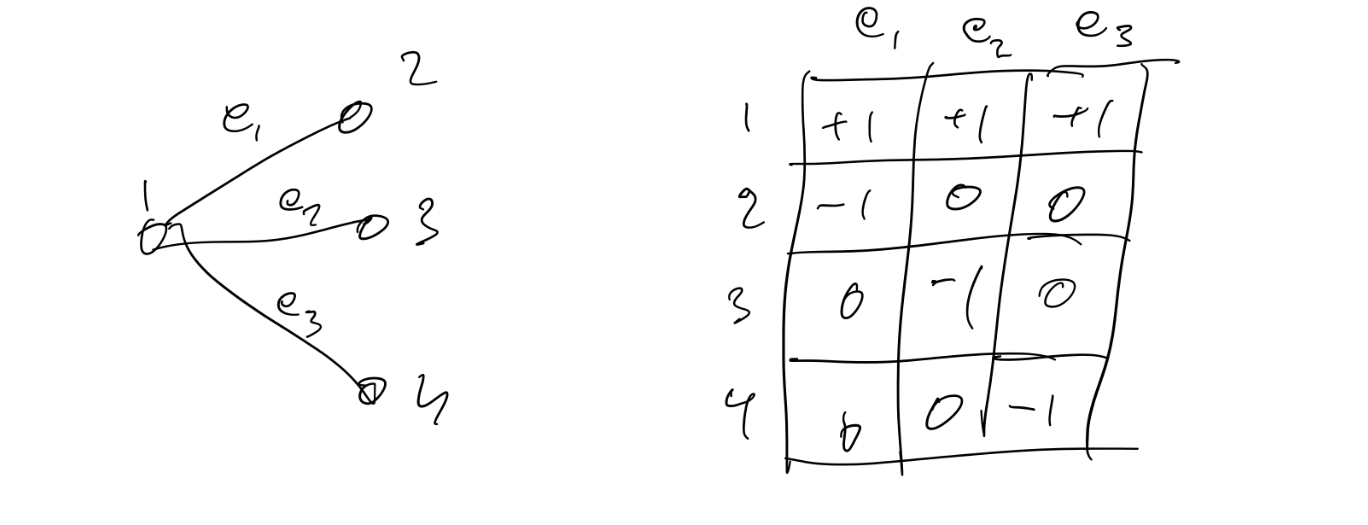
\includegraphics[width=0.7\textwidth]{fig/lecture6_incidence-example.jpeg}
  \caption{An example of a graph and its incidence matrix $B$.}
\label{fig:incidenceexample}
\end{figure}

In Chapter 1, we introduced the electrical flow routing  demand
$\dd\in\R^V$.
Let's call the electrical flow $\fftil\in\R^E$. The net flow
constraint requires $\BB\fftil = \dd$. By Ohm's Law,
$\fftil=\RR^{-1}\BB^\trp\xx$ for some voltage $x\in\R^V$ where
$\RR=\diag(\rr)$ and $\rr(e)=$ resistance of edge $e$. We showed (in
the exercises) that when $\dd \perp \matone$, there exists an voltage
$\xxtil\perp\matone$ s.t.\ $\fftil=\RR^{-1}\BB^\trp\xxtil$ and
$\BB\fftil = \dd$. This $\xxtil$ solves $\LL\xx=\dd$ where
$\LL=\BB\RR^{-1}\BB^\trp$.

And we also made the following claim.
\begin{claim}
  \begin{equation}
    \label{eq:argminflow}
    \fftil = \argmin_{\BB\ff=\dd} \ff^\trp\RR\ff \text{ where }
    \ff^\trp\RR\ff=\sum_e \rr(e)\ff(e)^2,
  \end{equation}
\end{claim}
You proved this in the exercises for Week 1. Let's recap the proof
briefly, just to get back into thinking about electrical flows.
\begin{proof}
Consider any $\ff\in\R^E$ s.t.\ $\BB\ff=\dd$. For any $\xx\in\R^V$, we have
\begin{align*}
	\frac{1}{2}\ff^\trp\RR\ff
	&= \frac{1}{2}\ff^\trp\RR\ff  - \xx^\trp(\underbrace{\BB\ff-\dd}_{\matzero}) \\
	&\geq \min_{\ff\in\R^E} \underbrace{\frac{1}{2}\ff^\trp\RR\ff  - \xx^\trp\BB\ff + \dd^\trp\xx}_{g(\ff)}  \\
	&= \dd^\trp\xx - \frac{1}{2}\xx^\trp\LL\xx
\end{align*}
since $\nabla_{\ff}g(\ff) = \matzero$ gives us $\ff=\RR^{-1}\BB^\trp\xx$. Thus, for all $\ff\in\R^E$ s.t.\ $\BB\ff=\dd$ and all $\xx\in\R^V$,
\begin{equation}
  \label{eq:flowsboundedbyvoltages}
\frac{1}{2}\ff^\trp\RR\ff \geq \dd^\trp\xx -
  \frac{1}{2}\xx^\trp\LL\xx.
\end{equation}
But for the electrical flow $\fftil$ and electrical voltage $\xxtil$, we have $\fftil=\RR^{-1}\BB^\trp\xxtil$ and $\LL\xxtil=\dd$. So
\[ \fftil^\trp\RR\fftil = \left(\RR^{-1}\BB^\trp\xxtil\right)^\trp\RR\left(\RR^{-1}\BB^\trp\xxtil\right) = \xxtil^\trp\BB\RR^{-1}\BB^\trp\xxtil = \xxtil^\trp\LL\xxtil  =\xxtil^\trp\dd. \]
Therefore,
\begin{equation}
   \label{eq:flowattainsvoltagevalue}
\frac{1}{2}\fftil^\trp\RR\fftil = \dd^\trp\xxtil -
\frac{1}{2}\xxtil^\trp\LL\xxtil.
\end{equation}
 By combining Equation~\eqref{eq:flowsboundedbyvoltages} and
 Equation~\eqref{eq:flowattainsvoltagevalue}, we see that for all
 $\ff$ s.t.\ $\BB \ff = \dd$,
 \[
 \frac{1}{2}\ff^\trp\RR\ff \geq \dd^\trp\xxtil -
\frac{1}{2}\xxtil^\trp\LL\xxtil = \frac{1}{2}\fftil^\trp\RR\fftil.
\]
Thus $\fftil$ is the minimum electrical energy flow among all flows
that route demand $\dd$, proving Equation~\eqref{eq:argminflow} holds.

The drawing below shows how the quantities line up:
\begin{figure}[H]
  \centering
     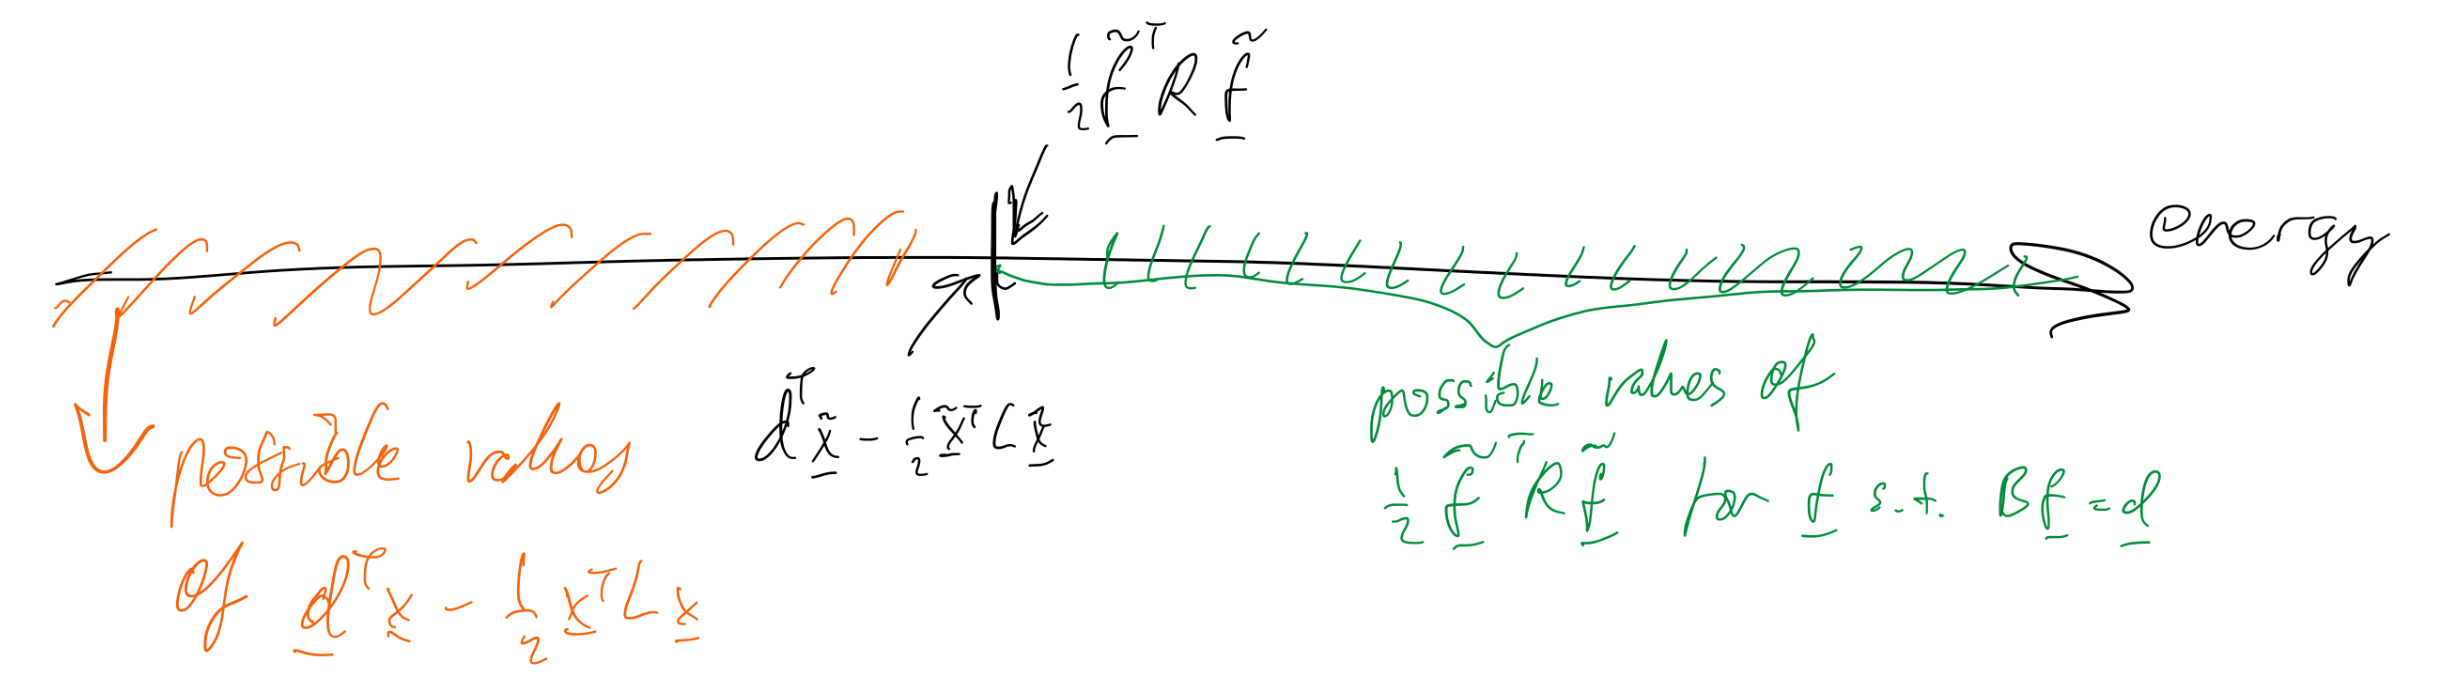
\includegraphics[width=\textwidth]{fig/lecture6_maxminfig.jpeg}
% \caption{}
\label{fig:regions}
\end{figure}
\end{proof}



\section{Effective Resistance}
Given a graph $G=(V,E)$, for any pair of vertices $(a,b)\in V$, we
want to compute the cost (or energy) of routing 1 unit of current
from $a$ to $b$. We call such cost the effective resistance between
$a$ and $b$, denoted by $\er(a,b)$. Recall for a single resistor
$r(a,b)$,
\[
  \text{energy} =r(a,b)f^2(a,b)=r(a,b)
  .
\]
So when we have a graph consisting of just one edge
$(a,b)$, the effective resistance is just $\er(a,b)=r(a,b)$.

In a general graph, we can also consider the energy required to route
one unit of current between two vertices.
For any pair $a,b\in V$, we have
\[ \er(a,b) = \min_{\BB\ff=\ee_b-\ee_a} \ff^\trp\RR\ff, \]
where $\ee_v \in \mathbb{R}^V$ is the indicator vector of $v$.
Note that the cost of routing $F$ units of flow from $a$ to $b$ will be $\er(a,b)\cdot F^2$.

Since $(\ee_b-\ee_a)^\trp\matone=0$, we know from the previous section
that $\er(a,b) = \fftil^\trp\RR\fftil$ where $\fftil$ is the
electrical flow.
Now we can write
$\LL\xxtil=\ee_b-\ee_a$ and $\xxtil=\LL^{\pinv}(\ee_b-\ee_a)$ for the
electrical voltages routing 1 unit of current from $a$ to $b$.
% where we let $\xxtil\perp\matone$ to use condition 3) of the
% pseudoinverse $\LL^{\pinv}$.
Now the energy of routing 1 unit of current from $a$ to $b$ is
\[ \er(a,b) = \fftil^\trp\RR\fftil = \xxtil^\trp\LL\xxtil =  (\ee_b-\ee_a)^\trp\LL^{\pinv}\LL\LL^{\pinv}(\ee_b-\ee_a) = (\ee_b-\ee_a)^\trp\LL^{\pinv}(\ee_b-\ee_a), \]
where the last equality is due to
$\LL^{\pinv}\LL\LL^{\pinv}=\LL^{\pinv}$.

\begin{remark}
  We have now seen several different expressions that all take on the
  same value: the energy of the electrical flow.
  It's useful to remind yourself what these are.
  Consider an electrical flow $\fftil$ routes demand $\dd$, and
  associated electrical voltages
  $\xxtil$.
  We know that $\BB \fftil = \dd$, and $\ff = \RR^{-1} \BB^{\trp}
  \xxtil$,
  and $\LL \xxtil = \dd$, where $\LL = \BB \RR^{-1} \BB^{\trp}$.
  And we have seen how to express the electrical energy using many
  different quantities:
  \[
     \fftil^\trp\RR\fftil  =  \xxtil^\trp\LL\xxtil = \dd^\trp \LL^{\pinv}
     \dd =\dd^\trp\xxtil = \fftil^{\trp}\BB^{\trp} \xxtil
   \]
\end{remark}

\begin{claim}
	Any PSD matrix $\AA$ has a PSD square root $\AA^{1/2}$ s.t.\ $\AA^{1/2}\AA^{1/2}=\AA$.
\end{claim}
\begin{proof}
	By the spectral theorem, $\AA = \sum_i \lambda_i\vv_i\vv_i^\trp$ where $\{\vv_i\}$ are orthonormal. Let $\AA^{1/2} = \sum_i \lambda_i^{1/2}\vv_i\vv_i^\trp$. Then
	\begin{align*}
		\AA^{1/2}\AA^{1/2}
		&= \left(\sum_i \lambda_i^{1/2}\vv_i\vv_i^\trp\right)^2 \\
		&= \sum_{i}\lambda_i \vv_i\vv_i^\trp\vv_i\vv_i^\trp + \sum_{i\neq j}\lambda_i \vv_i\vv_i^\trp\vv_j\vv_j^\trp \\
		&= \sum_i \lambda_i\vv_i\vv_i^\trp \\
	\end{align*}
	where the last equality is due to $\vv_i^\trp\vv_j = \delta_{ij}$. It's easy to see that $\AA^{1/2}$ is also PSD.
\end{proof}

Let $\LL^{+/2}$ be the square root of $\LL^{+}$. So
\[ \er(a,b) = (\ee_b-\ee_a)^\trp\LL^{\pinv}(\ee_b-\ee_a) = \|\LL^{+/2}(\ee_b-\ee_a)\|^2. \]

\paragraph{Example: Effective resistance in a path.}
Consider a path graph on vertices $V = \setof{1,2,3,\ldots, k+1}$,
with with resistances $\rr(1), \rr(2), \ldots, \rr(k)$ on
the edges of the path.
\begin{figure}[H]
  \centering
  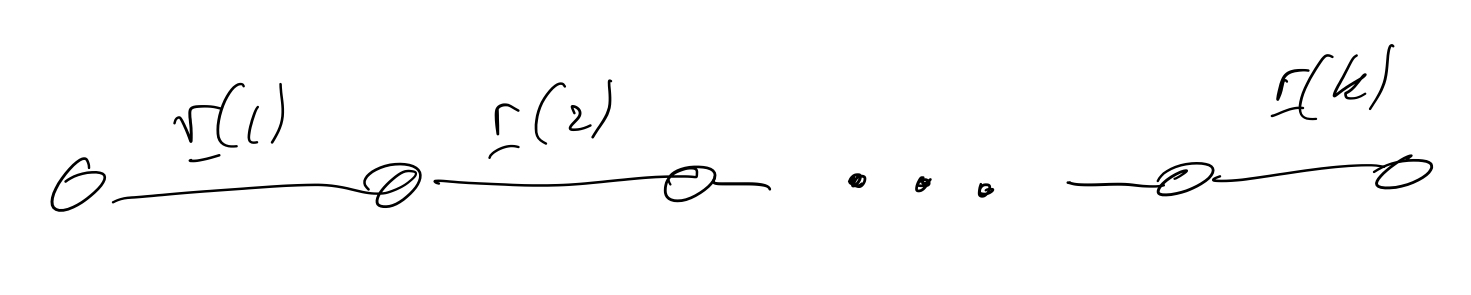
\includegraphics[width=0.6\textwidth]{fig/lecture6_seriesres.jpeg}
  \caption{A path graph with $k$ edges.}
\label{fig:seriesres}
\end{figure}
The effective resistance between the
endpoints is
\[
  \er(1,k+1) = \sum_{i = 1}^{k} \rr(i)
  \]
To see this, observe that to have 1 unit of flow going from vertex $1$ to vertex $k+1$, we must
have one unit flowing across each edge $i$.
Let $\DDelta(i)$ be the voltage difference across edge $i$, and $\ff(i)$ the
flow on the edge.
Then $1 = \ff(i) = \frac{\DDelta(i)}{\rr(i)}$, so that $\DDelta(i) =
\rr(i)$.
The electrical voltages are then $\xxtil \in \R^V$ where $\xxtil(i) =
\xxtil(1) + \sum_{j < i} \DDelta(j)$.
Hence the effective resistance is
\[\er(1,k+1) = \dd^{\trp}\xxtil=  (\ee_{k+1}-\ee_{1})^{\trp}\xxtil = \xxtil(k+1) -
  \xxtil(1) = \sum_{i = 1}^{k} \rr(i)
.
\]
This behavior is sometimes known as the fact that the resistance of
resistors adds up when they are connected in series.

\paragraph{Example: Effective resistance of parallel edges.}
So far, we have only considered graphs with at most one edge between
any two vertices. But that math also works if we allow a pair of
vertices to have multiple distinct edges connecting them. We refer to
this as \emph{multi-edges}.
Suppose we have a graph on just two vertices, $V = \setof{1,2}$, and
these are connected by $k$ parallel multi-edges with resistances
$\rr(1), \rr(2), \ldots, \rr(k)$.
\begin{figure}[H]
  \centering
  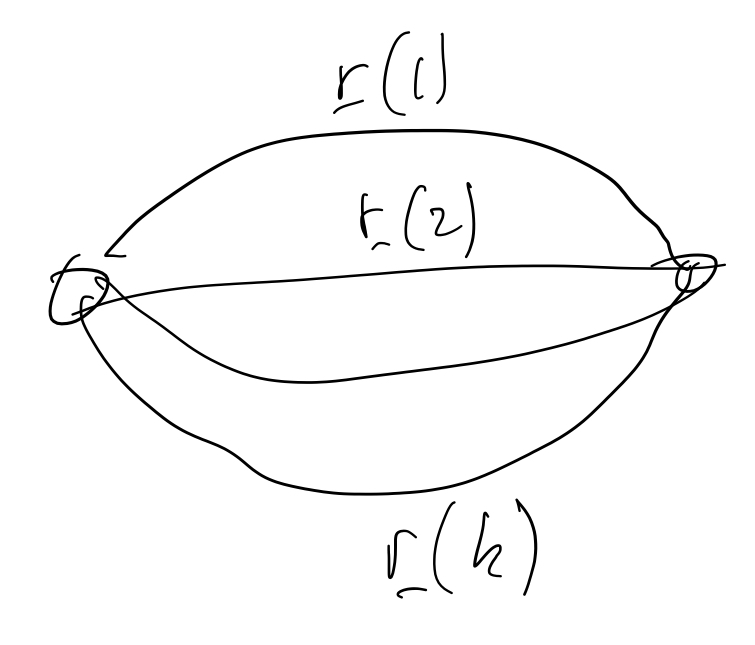
\includegraphics[width=0.3\textwidth]{fig/lecture6_parallelres.jpeg}
  \caption{A graph on just two vertices with $k$ parallel multiedges.}
\label{fig:parallelres}
\end{figure}
The effective resistance between the endpoints is
\[
  \er(1,2) =
  \frac{1}{\sum_{i = 1}^k 1/\rr(i)}
  .
\]
Let's see why.
Our electrical voltages $\xxtil \in \R^V$ can be described by just the voltage
difference $\Delta \in \R$ between vertex 1 and vertex 2, i.e. $\xxtil(2)
- \xxtil(1) = \Delta$.
which creates a flow on edge $i$ of $\fftil(i) = \Delta/\rr(i)$.
Thus the total flow from vertex 1 to vertex 2 is
$1 = \sum_{i} \Delta/\rr(i)$,
so that $\Delta =\frac{1}{\sum_{i = 1}^k 1/\rr(i)}$.
Meanwhile, the effective resistance is also
\[
\er(1,2) = (\ee_{2}-\ee_{1})^{\trp}\xxtil = \Delta =\frac{1}{\sum_{i = 1}^k 1/\rr(i)}
  \]
\subsection{Effective Resistance is a Distance}
\boxdef{
  \label{def:dist}
  Consider a weighted undirected graph $G$ with vertex set $V$.  We
  say function $d: V \times V \to \R$, which takes a pair of vertices
  and returns a real number, is a \emph{distance} if it satisfies
  \begin{enumerate}
  \item $d(a,a) = 0$ for all $a \in V$ \label{enu:distzero}
  \item $d(a,b) \geq 0$ for all $a,b \in V$. \label{enu:distnonneg}
  \item $d(a,b) = d(b,a)$ for all $a,b \in V$. \label{enu:distsym}
  \item $d(a,b) \leq d(a,c) + d(c,b)$ for all $a,b,c \in
    V$. \label{enu:disttri}
  \end{enumerate}
}
\begin{lemma}
  $\er$ is a distance.
\end{lemma}
Before proving this lemma, let's see a claim that will help us finish
the proof.
\begin{claim}
    \label{clm:voltageorder}
    Let $\LL \xxtil = \ee_b - \ee_a$.
    Then for all $\cc \in V$, we have $\xxtil(b) \geq \xxtil(c) \geq \xxtil(a)$.
  \end{claim}
  We only sketch a proof of this claim:
  \begin{proof}[Proof sketch]
    Consider any $c \in V$, where $c\neq a,b$.
    Now $(\LL \xxtil)(c) = 0$, i.e.
    \[
      \left( \sum_{(u,c)} \ww(u,c) \right) \xxtil(c) - \left(
        \sum_{(u,c)} \ww(u,c) \xxtil(u) \right) = 0
    \]
    Rearranging $ \xxtil(c) = \frac{\sum_{(u,c)} \ww(u,c) \xxtil(u)
    }{\sum_{(u,c)} \ww(u,c)}$.
   This tells us that $\xxtil(c)$ is a weighted average of the
   voltages of its neighbors. From this, we can show that $\xxtil(a)$
   and $\xxtil(b)$ are the extreme values.
  \end{proof}
\begin{proof}
  It is easy to check that conditions
  \ref{enu:distzero}, \ref{enu:distnonneg}, and \ref{enu:distsym} of Definition~\ref{def:dist} are satisfied by
  $\er$.
  Let us confirm condition~\ref{enu:disttri}.

  For any $u,v$, let $\xxtil_{u,v} = \LL^\pinv ( -\ee_u + \ee_v )$.
  Then
  \[
    \xxtil_{a,b} = \LL^\pinv ( -\ee_a+ \ee_b)
  =  \LL^\pinv ( -\ee_a + \ee_c - \ee_c  + \ee_b)
  = \xxtil_{a,c} + \xxtil_{c,b}
  .
\]
Thus,
\begin{align*}
  \er(a,b) =  ( -\ee_a+ \ee_b)^\trp \xxtil_{a,b}
  &=  ( -\ee_a+ \ee_b)^\trp(\xxtil_{a,c} + \xxtil_{c,b})
  \\
  &= -\xxtil_{a,c}(a) + \xxtil_{a,c}(b) -\xxtil_{c,b}(a) +
  \xxtil_{c,b}(b)
  \\
   &\leq -\xxtil_{a,c}(a) + \xxtil_{a,c}(c) -\xxtil_{c,b}(c) +
     \xxtil_{c,b}(b).
\end{align*}
where in the last line we applied Claim~\ref{clm:voltageorder} to show
that $\xxtil_{a,c}(b) \leq \xxtil_{a,c}(c)$ and ${ -\xxtil_{c,b}(a) \leq  -\xxtil_{c,b}(c)}$.
\end{proof}



%%% Local Variables:
%%% mode: latex
%%% TeX-master: "main"
%%% TeX-engine: 
%%% End: